\chapter{Phylogenetic analysis}

Because of ease of use, I chose \emph{NCBI BLAST} on \emph{UniProtKB/SwissProt} database for finding 6 mammal and a bird sequence of my protein \emph{DLG3}.
I chose the mentioned databases, because they are well supported, and validated by many researchers.

I have chosen the following sequences (6 mammal, 1 bird):
\begin{itemize}
\item \href{https://blast.ncbi.nlm.nih.gov/Blast.cgi#alnHdr_223590196}{Q12959.2}
\item \href{https://blast.ncbi.nlm.nih.gov/Blast.cgi#alnHdr_59797853}{Q811D0.1}

\item \href{https://blast.ncbi.nlm.nih.gov/Blast.cgi#alnHdr_182667930}{Q8BVD5.2}
\item \href{https://blast.ncbi.nlm.nih.gov/Blast.cgi#alnHdr_67460767}{Q5RDQ2.1}

\item \href{https://blast.ncbi.nlm.nih.gov/Blast.cgi#alnHdr_2497505}{ 	Q62696.1}
\item \href{https://blast.ncbi.nlm.nih.gov/Blast.cgi#alnHdr_71658825}{P78352.3}

\item \href{https://www.ncbi.nlm.nih.gov/protein/1708495?report=genbank&log\$=prottop&blast_rank=2&RID=33MZJTCK014}{P51527.1}
\end{itemize}

I have combined these sequences into one fasta file, \url{~/files/ex7.fasta}.
I used \href{http://www.bioinformatics.org/sms2/rev_trans.html}{\emph{Bioinformatics.org} SMS} to translate the sequences to mRNA sequences.

I multiple aligned both sequence file, using \href{http://www.genome.jp/tools-bin/clustalw}{Genome.jp CLUSTALW}, resulting in \url{~/files/ex7align.fasta}.
I also used this website's tool to generate the \emph{Rooted phylogenetic tree (UPGMA)}, with and without the branch length representing the predicted distance between species.

I also applied the suggested \textbf{R} program to compare the results.
The comparison on Figure \ref{comapre1}.
In conclusion it can be said that the original PDZ (1, 2, 3) sites are very close to each other (\texttt{Q811D0.1}, \texttt{Q62696.1}, \texttt{Q12959.2}) from phylogenetical aspect.



\begin{figure}
\centering
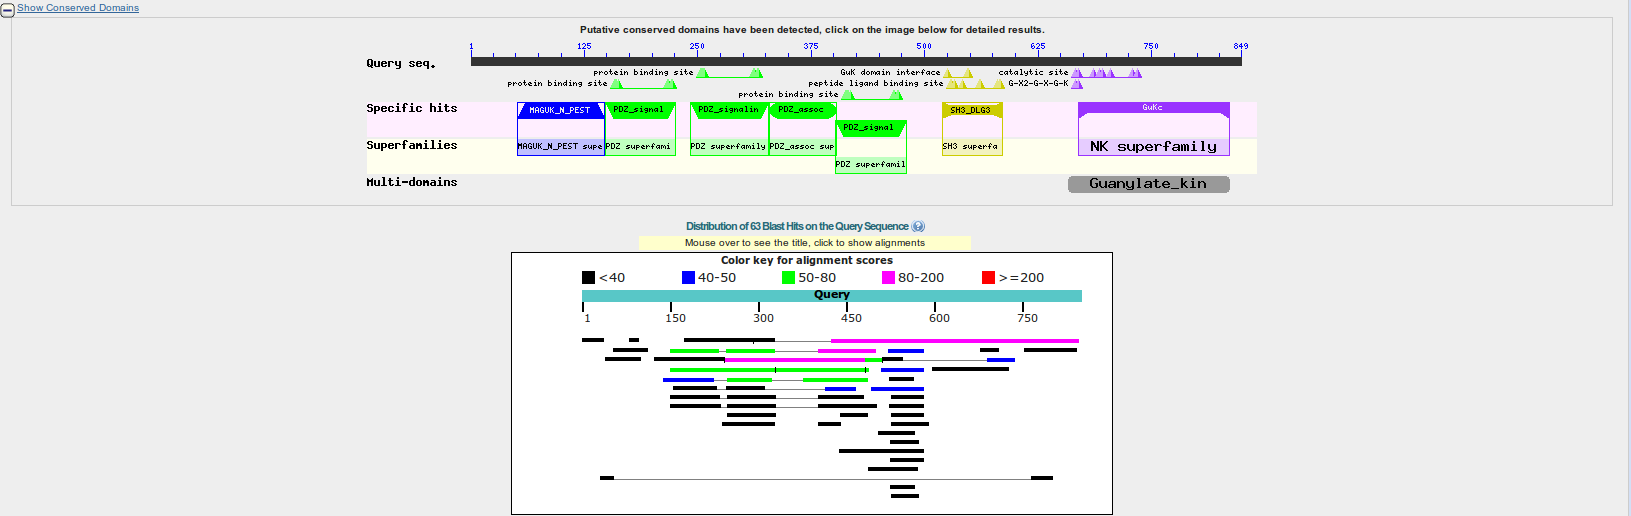
\includegraphics[width=\textwidth]{birdalign.png}
\caption{Searching for the DLG3 sequence among proteins of birds results in a poor matching, I have chosen the Sequence with the highest \texttt{Ident} value (53 \%)-}
\label{bird}
\end{figure}

\begin{figure}
\centering
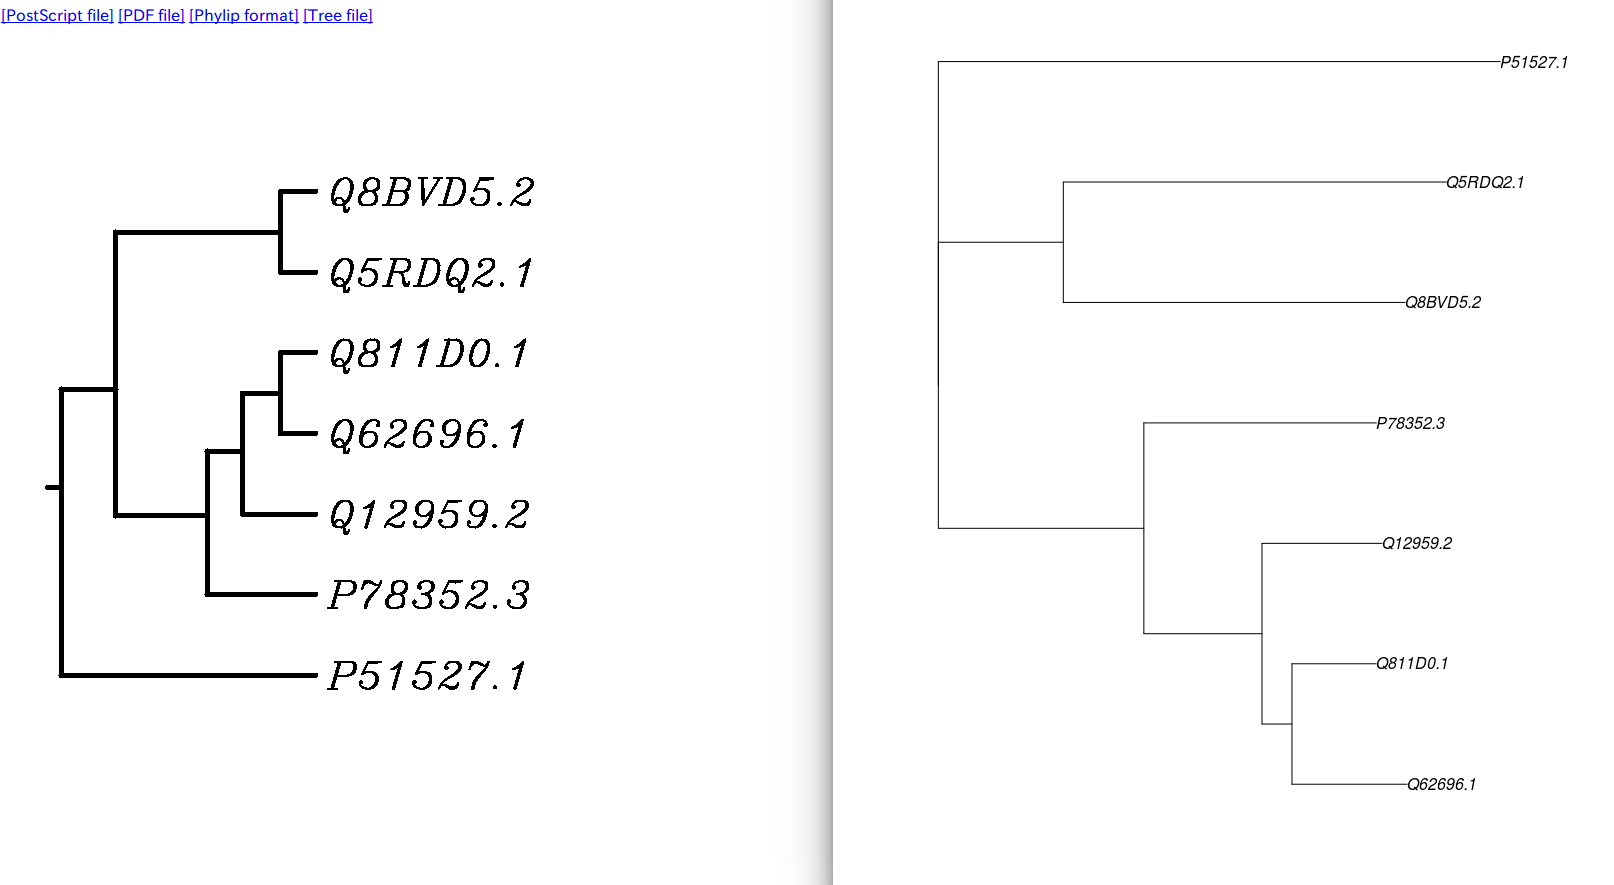
\includegraphics[width=\textwidth]{rcompare.png}
\caption{Comparing the results of \emph{R} and \emph{Genome.jp}. Except the ordering (which can be cosidered as invariant) these trees are identical. Therefore in the following I use \emph{Genome.jp} because of the user-friendly interface.}
\label{comapre1}
\end{figure}

\begin{figure}
\centering
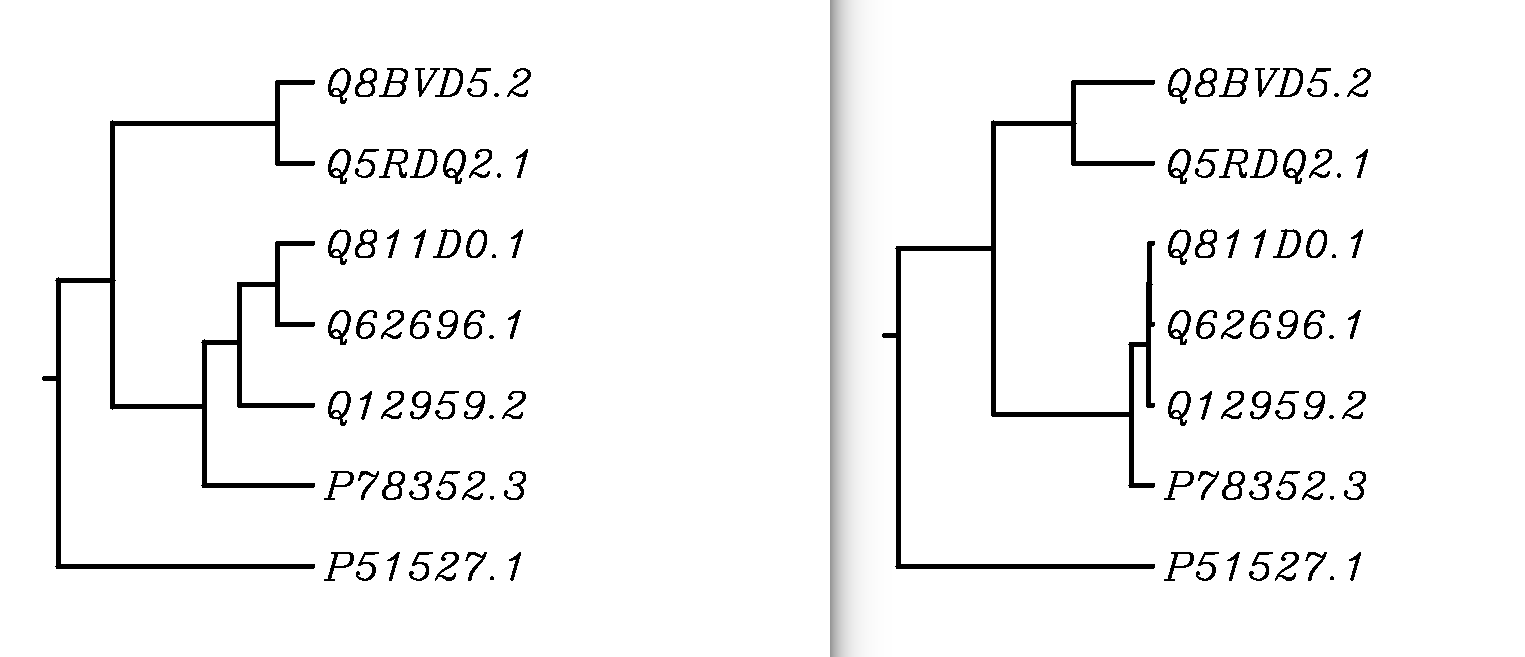
\includegraphics[width=\textwidth]{nodist-dist.png}
\caption{\emph{On the left:} Tree, showing equidistant ascension. \emph{On the right:} Tree, which branches represent the distance of the corresponding sequences. It can be seen, that the original PDZ domains fall very close to each others.}
\label{comapre2}
\end{figure}

